% Created 2022-11-16 Wed 10:41
% Intended LaTeX compiler: pdflatex
\documentclass[presentation]{beamer}
\usepackage[utf8]{inputenc}
\usepackage[T1]{fontenc}
\usepackage{fontspec}
\usepackage{xcolor}
\usepackage{hyperref}
% features: (acronym underline par-sep beamer image .missing-koma)
\newcommand{\acr}[1]{\protect\textls*[110]{\scshape #1}}
\newcommand{\acrs}{\protect\scalebox{.91}[.84]{\hspace{0.15ex}s}}
\usepackage[normalem]{ulem}
\setlength{\parskip}{\baselineskip}
\setlength{\parindent}{0pt}

\usepackage{graphicx}
\usepackage{scrextend}
% end features

%% make document follow Emacs theme

\definecolor{obg}{HTML}{2E3440}
\definecolor{ofg}{HTML}{ECEFF4}

% heading colours
\definecolor{documentTitle}{HTML}{81A1C1}
\definecolor{documentInfo}{HTML}{81A1C1}
\definecolor{level1}{HTML}{81A1C1}
\definecolor{level2}{HTML}{B48EAD}
\definecolor{level3}{HTML}{5D80AE}
\definecolor{level4}{HTML}{a0b8d0}
\definecolor{level5}{HTML}{c6aac1}
\definecolor{level6}{HTML}{c0d0e0}
\definecolor{level7}{HTML}{d9c6d6}
\definecolor{level8}{HTML}{e5ecf2}

% textual elements

\definecolor{link}{HTML}{81A1C1}
\colorlet{url}{link}
\definecolor{cite}{HTML}{98c1c0}
\definecolor{itemlabel}{HTML}{81A1C1}
\definecolor{code}{HTML}{D08770}
\definecolor{verbatim}{HTML}{A3BE8C}

\DeclareTextFontCommand{\texttt}{\color{code}\ttfamily}

\let\oldverb\verb
\def\verb{\bgroup\color{verbatim}\oldverb}
\makeatletter
\let\verb@oldegroup\verb@egroup
\def\verb@egroup{\verb@oldegroup\egroup}
\makeatother

% beamer

\definecolor{builtin}{HTML}{81A1C1}
\definecolor{varname}{HTML}{D8DEE9}

\NewCommandCopy{\oldusetheme}{\usetheme}
\renewcommand*{\usetheme}[2][]{\oldusetheme[#1]{#2}
  \setbeamercolor{title separator}{fg=documentTitle}
  \setbeamercolor{progress bar}{fg=documentTitle}
  \setbeamercolor{progress bar in head/foot}{fg=documentTitle}
  \setbeamercolor{progress bar in section page}{fg=documentTitle}

  \setbeamercolor{normal text}{fg=ofg, bg=obg}
  \setbeamercolor{alerted text}{fg=varname}
  \setbeamercolor*{item}{fg=itemlabel}
  \setbeamercolor{block title}{fg=level3, bg=}
}

\usepackage{etoolbox}
\makeatletter
\patchcmd{\beamer@section}{%
  \edef\insertsectionhead{\noexpand\hyperlink{Navigation\the\c@page}{\unexpanded{#1}}}}{%
  \edef\insertsectionhead{\begingroup\noexpand\hypersetup{hidelinks}\noexpand\hyperlink{Navigation\the\c@page}{\unexpanded{#1}}\endgroup}}
\makeatother

% code blocks

\definecolor{codebackground}{HTML}{373E4C}
\colorlet{EFD}{ofg}
\definecolor{codeborder}{HTML}{404654}

%% end customisations

\usetheme[progressbar=foot]{metropolis}
\author{Ellis Kenyő}
\date{\today}
\title{Git}
\subtitle{(Or how I learned to stop worrying and love version control)}
\titlegraphic{
\includegraphics[height=1.5cm]{git_icon.png}}
\usepackage{pgfpages}
\setbeameroption{show notes on second screen=right}
\colorlet{greenyblue}{blue!70!green}
\colorlet{blueygreen}{blue!40!green}
\providecolor{link}{named}{greenyblue}
\providecolor{cite}{named}{blueygreen}
\hypersetup{
  pdfauthor={Ellis Kenyő},
  pdftitle={Git},
  pdfkeywords={},
  pdfsubject={},
  pdfcreator={Emacs 28.2 (Org mode 9.6-pre)},
  pdflang={English},
  breaklinks=true,
  colorlinks=true,
  linkcolor=,
  urlcolor=link,
  citecolor=cite
}
\urlstyle{same}

% Setup for code blocks [1/2]

\usepackage{fvextra}

\fvset{%
  commandchars=\\\{\},
  highlightcolor=white!95!black!80!blue,
  breaklines=true,
  breaksymbol=\color{white!60!black}\tiny\ensuremath{\hookrightarrow}}

% Make line numbers smaller and grey.
\renewcommand\theFancyVerbLine{\footnotesize\color{black!40!white}\arabic{FancyVerbLine}}

\usepackage{xcolor}

% In case engrave-faces-latex-gen-preamble has not been run.
\providecolor{EfD}{HTML}{f7f7f7}
\providecolor{EFD}{HTML}{28292e}

% Define a Code environment to prettily wrap the fontified code.
\usepackage[breakable,xparse]{tcolorbox}
\DeclareTColorBox[]{Code}{o}%
{colback=EfD!98!EFD, colframe=EfD!95!EFD,
  fontupper=\footnotesize\setlength{\fboxsep}{0pt},
  colupper=EFD,
  IfNoValueTF={#1}%
  {boxsep=2pt, arc=2.5pt, outer arc=2.5pt,
    boxrule=0.5pt, left=2pt}%
  {boxsep=2.5pt, arc=0pt, outer arc=0pt,
    boxrule=0pt, leftrule=1.5pt, left=0.5pt},
  right=2pt, top=1pt, bottom=0.5pt,
  breakable}

% Support listings with captions
\usepackage{float}
\floatstyle{plain}
\newfloat{listing}{htbp}{lst}
\newcommand{\listingsname}{Listing}
\floatname{listing}{\listingsname}
\newcommand{\listoflistingsname}{List of Listings}
\providecommand{\listoflistings}{\listof{listing}{\listoflistingsname}}


% Setup for code blocks [2/2]: syntax highlighting colors

\newcommand\efstrut{\vrule height 2.1ex depth 0.8ex width 0pt}
\definecolor{EFD}{HTML}{ECEFF4}
\definecolor{EfD}{HTML}{2E3440}
\newcommand{\EFD}[1]{\textcolor{EFD}{#1}} % default
\newcommand{\EFvp}[1]{#1} % variable-pitch
\definecolor{EFh}{HTML}{4C566A}
\newcommand{\EFh}[1]{\textcolor{EFh}{#1}} % shadow
\definecolor{EFsc}{HTML}{A3BE8C}
\newcommand{\EFsc}[1]{\textcolor{EFsc}{#1}} % success
\definecolor{EFw}{HTML}{EBCB8B}
\newcommand{\EFw}[1]{\textcolor{EFw}{#1}} % warning
\definecolor{EFe}{HTML}{BF616A}
\newcommand{\EFe}[1]{\textcolor{EFe}{#1}} % error
\definecolor{EFl}{HTML}{81A1C1}
\newcommand{\EFl}[1]{\textcolor{EFl}{\textbf{#1}}} % link
\definecolor{EFlv}{HTML}{ee82ee}
\newcommand{\EFlv}[1]{\textcolor{EFlv}{\textbf{#1}}} % link-visited
\definecolor{EFhi}{HTML}{191C25}
\definecolor{Efhi}{HTML}{81A1C1}
\newcommand{\EFhi}[1]{\colorbox{Efhi}{\efstrut{}\textcolor{EFhi}{#1}}} % highlight
\definecolor{EFc}{HTML}{6f7787}
\newcommand{\EFc}[1]{\textcolor{EFc}{#1}} % font-lock-comment-face
\definecolor{EFcd}{HTML}{6f7787}
\newcommand{\EFcd}[1]{\textcolor{EFcd}{#1}} % font-lock-comment-delimiter-face
\definecolor{EFs}{HTML}{A3BE8C}
\newcommand{\EFs}[1]{\textcolor{EFs}{#1}} % font-lock-string-face
\definecolor{EFd}{HTML}{78808f}
\newcommand{\EFd}[1]{\textcolor{EFd}{#1}} % font-lock-doc-face
\definecolor{EFm}{HTML}{81A1C1}
\newcommand{\EFm}[1]{\textcolor{EFm}{#1}} % font-lock-doc-markup-face
\definecolor{EFk}{HTML}{81A1C1}
\newcommand{\EFk}[1]{\textcolor{EFk}{#1}} % font-lock-keyword-face
\definecolor{EFb}{HTML}{81A1C1}
\newcommand{\EFb}[1]{\textcolor{EFb}{#1}} % font-lock-builtin-face
\definecolor{EFf}{HTML}{88C0D0}
\newcommand{\EFf}[1]{\textcolor{EFf}{#1}} % font-lock-function-name-face
\definecolor{EFv}{HTML}{D8DEE9}
\newcommand{\EFv}[1]{\textcolor{EFv}{#1}} % font-lock-variable-name-face
\definecolor{EFt}{HTML}{8FBCBB}
\newcommand{\EFt}[1]{\textcolor{EFt}{#1}} % font-lock-type-face
\definecolor{EFo}{HTML}{81A1C1}
\newcommand{\EFo}[1]{\textcolor{EFo}{#1}} % font-lock-constant-face
\definecolor{EFwr}{HTML}{EBCB8B}
\newcommand{\EFwr}[1]{\textcolor{EFwr}{#1}} % font-lock-warning-face
\definecolor{EFnc}{HTML}{81A1C1}
\newcommand{\EFnc}[1]{\textcolor{EFnc}{\textbf{#1}}} % font-lock-negation-char-face
\definecolor{EFpp}{HTML}{81A1C1}
\newcommand{\EFpp}[1]{\textcolor{EFpp}{\textbf{#1}}} % font-lock-preprocessor-face
\definecolor{EFrc}{HTML}{81A1C1}
\newcommand{\EFrc}[1]{\textcolor{EFrc}{\textbf{#1}}} % font-lock-regexp-grouping-construct
\definecolor{EFrb}{HTML}{81A1C1}
\newcommand{\EFrb}[1]{\textcolor{EFrb}{\textbf{#1}}} % font-lock-regexp-grouping-backslash
\definecolor{Efob}{HTML}{373E4C}
\newcommand{\EFob}[1]{\colorbox{Efob}{\efstrut{}#1}} % org-block
\definecolor{EFobb}{HTML}{6f7787}
\definecolor{Efobb}{HTML}{373E4C}
\newcommand{\EFobb}[1]{\colorbox{Efobb}{\efstrut{}\textcolor{EFobb}{#1}}} % org-block-begin-line
\definecolor{EFobe}{HTML}{6f7787}
\definecolor{Efobe}{HTML}{373E4C}
\newcommand{\EFobe}[1]{\colorbox{Efobe}{\efstrut{}\textcolor{EFobe}{#1}}} % org-block-end-line
\definecolor{EFOa}{HTML}{81A1C1}
\newcommand{\EFOa}[1]{\textcolor{EFOa}{\textbf{#1}}} % outline-1
\definecolor{EFOb}{HTML}{B48EAD}
\newcommand{\EFOb}[1]{\textcolor{EFOb}{\textbf{#1}}} % outline-2
\definecolor{EFOc}{HTML}{5D80AE}
\newcommand{\EFOc}[1]{\textcolor{EFOc}{\textbf{#1}}} % outline-3
\definecolor{EFOd}{HTML}{a0b8d0}
\newcommand{\EFOd}[1]{\textcolor{EFOd}{\textbf{#1}}} % outline-4
\definecolor{EFOe}{HTML}{c6aac1}
\newcommand{\EFOe}[1]{\textcolor{EFOe}{\textbf{#1}}} % outline-5
\definecolor{EFOf}{HTML}{c0d0e0}
\newcommand{\EFOf}[1]{\textcolor{EFOf}{\textbf{#1}}} % outline-6
\definecolor{EFOg}{HTML}{d9c6d6}
\newcommand{\EFOg}[1]{\textcolor{EFOg}{\textbf{#1}}} % outline-7
\definecolor{EFOh}{HTML}{e5ecf2}
\newcommand{\EFOh}[1]{\textcolor{EFOh}{\textbf{#1}}} % outline-8
\definecolor{EFhn}{HTML}{B48EAD}
\newcommand{\EFhn}[1]{\textcolor{EFhn}{\textbf{#1}}} % highlight-numbers-number
\definecolor{EFhq}{HTML}{81A1C1}
\newcommand{\EFhq}[1]{\textcolor{EFhq}{#1}} % highlight-quoted-quote
\definecolor{EFhs}{HTML}{8FBCBB}
\newcommand{\EFhs}[1]{\textcolor{EFhs}{#1}} % highlight-quoted-symbol
\definecolor{EFrda}{HTML}{81A1C1}
\newcommand{\EFrda}[1]{\textcolor{EFrda}{#1}} % rainbow-delimiters-depth-1-face
\definecolor{EFrdb}{HTML}{B48EAD}
\newcommand{\EFrdb}[1]{\textcolor{EFrdb}{#1}} % rainbow-delimiters-depth-2-face
\definecolor{EFrdc}{HTML}{A3BE8C}
\newcommand{\EFrdc}[1]{\textcolor{EFrdc}{#1}} % rainbow-delimiters-depth-3-face
\definecolor{EFrdd}{HTML}{5D80AE}
\newcommand{\EFrdd}[1]{\textcolor{EFrdd}{#1}} % rainbow-delimiters-depth-4-face
\definecolor{EFrde}{HTML}{8FBCBB}
\newcommand{\EFrde}[1]{\textcolor{EFrde}{#1}} % rainbow-delimiters-depth-5-face
\definecolor{EFrdf}{HTML}{81A1C1}
\newcommand{\EFrdf}[1]{\textcolor{EFrdf}{#1}} % rainbow-delimiters-depth-6-face
\definecolor{EFrdg}{HTML}{B48EAD}
\newcommand{\EFrdg}[1]{\textcolor{EFrdg}{#1}} % rainbow-delimiters-depth-7-face
\definecolor{EFrdh}{HTML}{A3BE8C}
\newcommand{\EFrdh}[1]{\textcolor{EFrdh}{#1}} % rainbow-delimiters-depth-8-face
\definecolor{EFrdi}{HTML}{5D80AE}
\newcommand{\EFrdi}[1]{\textcolor{EFrdi}{#1}} % rainbow-delimiters-depth-9-face
\begin{document}

\maketitle

\note{Notes
\tiny

Welcome to ``Git (Or how I learned to stop worrying and love version control)''; a talk on what git is, how to use it, how we \emph{should} use it and later how we can interact with the wider community. After this, I hope you will come away with something; and hopefully a thirst for digging deeper into using git. During the talk there will some pre-computed code examples but all of the examples have been run as-is with no external scripts/tools so anything in here should work.

There will be time at the end to ask any questions, just to ensure that I actually finish the workshop.
\normalsize}

\section{What is Git?}
\label{sec:org0a462f7}
\begin{frame}[label={sec:orgdb40019},fragile]{Overview}
 \begin{itemize}
\item Short answer; snapshot tracker
\item \href{https://www.git-scm.com/book/en/v2/Getting-Started-What-is-Git\%3F}{Long answer}
\item \href{https://www.youtube.com/watch?v=MYP56QJpDr4\&t=0s}{\texttt{unsigned long} answer}
\end{itemize}

\note{Notes
\tiny

Git is a distributed version control tool for source code management. What does that mean in English?

In the simplest terms, a version control tool is a tool for handling changes in files by storing the changes in files between generations. git (unlike other existing version control tools) doesn't store diffs/changes, it stores \emph{snapshots} rather then diffs. Think of it like time machine, each new ``snapshot'' of a file or files is called a commit. We'll dig more into these shortly.

The other links included are a short intro article expanding some basics, and a talk called ``Git From the Bits Up'' which demonstrates building a git directory without using git.}
\end{frame}

\begin{frame}[label={sec:orgd5928a0},fragile]{Terms}
 \begin{definition}[Commit]
verb: The action of storing a new snapshot

noun: A point in git history; a snapshot of a file or files
\end{definition}

\begin{definition}[Repository]
Also called repo; an object database along with their reachable objects
\end{definition}

\begin{definition}[Branch]
A subset of commits
\end{definition}

\begin{definition}[Push]
A series of operations to submit local changes to a remote repo
\end{definition}

\begin{definition}[Pull]
A series of operations to retrieve remote changes and add them to your local repo
\end{definition}

Source: \url{https://git-scm.com/docs/gitglossary}

\note{Notes
\tiny

Included here are some terms that occur during the presentation or often enough in general git usage to warrant a definition. Included at the bottom is a link to where I based these from, along with definitions for basically anything you're likely to encounter with git, which I'd recommend at least skimming to get definitions to things you might have come across and not been sure of.

Starting at the top, we have a commit; which is used both as a noun and a verb. The noun sense refers to a single snapshot of a file or files within the history of the current repository. More concretely it refers to a ``commit object'', which is an object (a hashed file inside the git repo) which stores the commit as well as metadata such as committer, author etc. This will be explored in more detail in the next slide.
The verb sense is simply the act of creating a commit.

Then we have a repository or repo; simply put this is just a group of files that also contains a correctly structured \texttt{.git} folder containing all the objects (including commits, branch data, etc)

Next we have a ``branch'', which fits with the idea of everything operating around a tree and represents an independent set of commits. A repo can have any number of branches, the only limit would come down to limitations of the file system in which the repo lies. The most recent commit on a branch is called the tip, and has a reference called ``head''.

Push/pull are operations performed by their respective CLI invocations and refer to taking changes from your local repo and pushing them to a remote repo; and vice versa.

\normalsize}
\end{frame}

\section{Commits}
\label{sec:orgecde87f}
\begin{frame}[label={sec:orgd59d870},fragile]{What \emph{is} a commit?}
 \tiny

\begin{Code}
\begin{Verbatim}
\color{EFD}\EFk{import} hashlib, zlib, os
\EFv{string\_to\_hash} = \EFs{'I am a file'}
\EFv{header} = \EFs{"blob "} + \EFb{str}(\EFb{len}(string\_to\_hash)) + \EFs{"\char92{}0"}
\EFv{blob} = (header + string\_to\_hash).encode(\EFs{'utf8'})
\EFv{sha} = hashlib.sha1(blob).hexdigest()
\EFv{git\_object} = f\EFs{".git/objects/}\{sha[:2]\}\EFs{/}\{sha[2:]\}\EFs{"}
os.makedirs(os.path.dirname(git\_object), exist\_ok=\EFo{True})
\EFk{with} \EFb{open}(git\_object, \EFs{'wb'}) \EFk{as} f:
    f.write(zlib.compress(blob))

\EFk{return} f\EFs{"Wrote: }\{git\_object\}\EFs{"}
\end{Verbatim}
\end{Code}

\begin{verbatim}
Wrote: .git/objects/1f/5614948c014b5b8284aa0504fdfa770ea01dce
\end{verbatim}


\begin{Code}
\begin{Verbatim}
\color{EFD}\EFt{git} cat-file -p \EFs{'1f56'}
\end{Verbatim}
\end{Code}

\begin{verbatim}
I am a file
\end{verbatim}


\href{https://www.youtube.com/watch?v=0g9BcZvQbXU}{Source}

\note{Notes
\tiny

I mentioned before what a commit is abstractly; a single snapshot in history. But that doesn't really help to understand what it is.

So I've used a trivial example to demonstrate me creating a new object in the git database for the string 'I am a file'. Skimming line-by-line for those that might not be familiar with Python:

L1: Importing libraries for hashing and general OS tasks

L2: Creating the string to hash

L3-5: Creating the actual object, which looks like ``blob <string length> <null terminator> <value of the object>'', then SHA1 hashing it

L6: Creating a variable for the file on disk to store in which is \texttt{.git/objects} then the first 2 characters of the hash, then everything from the second character onwards (this is done to prevent issues on file systems that don't like thousands of files in a directory)

L7: Create the path on disk (so we can write to the file)

L8-9: Open the file as writable in binary format then write the zlib-compressed hash

L11: Print the filename

And just like that, we have created an object in the database! We can prove that with the second example, which looks up a file in the git database by the hash and returns the contents, which is the original string we setup.

A commit is an object like the one created above, just with extra metadata.

\normalsize}
\end{frame}

\begin{frame}[label={sec:org23842b3},fragile,shrink=40]{OK, so \emph{how} do I make a commit?}
 \begin{columns}
\begin{column}{0.9\columnwidth}
\begin{block}{Creating commit}
\begin{Code}
\begin{Verbatim}
\color{EFD}\EFt{rm} -rf sample .git/ \&\& \EFt{git} init
\EFt{echo} \EFs{"Status before: "}
\EFt{git} status --short
\EFt{echo} \EFs{"I am a file"} > sample

\EFt{echo} \EFs{"Status after creating: "}
\EFt{git} status --short

\EFt{echo} \EFs{"Status after adding: "}
\EFt{git} add sample
\EFt{git} status --short

\EFt{echo} -e \EFs{"\char92{}n"}

\EFt{git} commit -m \EFs{"Initial commit"} --no-gpg-sign
\end{Verbatim}
\end{Code}

\begin{Code}
\begin{Verbatim}
\color{EFD}Initialized empty Git repository\EFk{ in} /tmp/test/.git/
Status before: 
?? file
Status after creating: 
?? file
?? sample
Status after adding: 
A  sample
?? file


\EFrda{[}master \EFrdb{(}root-commit\EFrdb{)} 467b20d\EFrda{]} Initial commit
 \EFhn{1} file changed, \EFhn{1} insertion\EFrda{(}+\EFrda{)}
 create mode \EFhn{100644} sample
\end{Verbatim}
\end{Code}
\end{block}
\end{column}

\begin{column}{0.9\columnwidth}
\begin{block}{Printing the object}
\begin{Code}
\begin{Verbatim}
\color{EFD}\EFt{git} cat-file -p \$\EFrda{(}\textcolor[HTML]{483d8b}{\textbf{git log -n 1 --pretty=format:\%H}}\EFrda{)}
\end{Verbatim}
\end{Code}

\begin{Code}
\begin{Verbatim}
\color{EFD}tree 446377584578f1a54bb90edaa39b144d658c2ba4
author Ellis Kenyő <me@elken.dev> \EFhn{1668595275} +0000
committer Ellis Kenyő <me@elken.dev> \EFhn{1668595275} +0000

Initial commit
\end{Verbatim}
\end{Code}
\end{block}
\end{column}
\end{columns}

\href{https://git-scm.com/docs/git-status\#\_short\_format}{Git status short format}

\note{Notes
\tiny

Obviously that process is quite tedious, but luckily git performs that for us (along with other cool things like redundancy checks) so how do we make a commit otherwise?

Well, we can just use the git CLI to create commits. I'm sure you've all done this before, but just so we're all on the same page let's step through the example above.

First we recreate our environment and run \texttt{git status -{}-short} to give us the short version of the status (mostly to just save screen space, feel free to use the normal \texttt{git status} when running for yourself)

Then, we create a file with the content ``I am a file'' and run status again.

What's changed? Now, we see the file we created prefixed with two question marks. These two characters represent first the status of the index then the status of the working tree. For a more detailed explanation, please see the link for ``git status short format''.

For our purposes though, the question marks simply mean the file is untracked. Any changes we make on it are not part of the git object database.

After we use \texttt{git add} on it, we now have a single A on the left side and nothing on the other (the gap is important). This means the file has been added, but not yet committed. Any changes are not persisted to the git object database.

After that, we commit the change and get the object from the database to inspect it. As you can see, it's the same as the object we created before just with extra metadata.

\normalsize}
\end{frame}


\begin{frame}[label={sec:org576ed27}]{How do I write commits?}
\begin{block}{Summary}
\begin{itemize}
\item Start with a short summary followed by a blank line
\item Body text should be wrapped to 72 characters
\item Use imperative mood
\item Use \href{https://www.conventionalcommits.org/en/v1.0.0/\#summary}{conventional commits} where possible (scopes \& types tbd)
\item The body should explain why \& how, not what
\item Include the jira ticket
\end{itemize}
\end{block}

\note{Notes
\tiny

Now that we know \emph{what} a commit is, we can come up to a much higher level and talk about writing commits. There are countless pages, books, articles and blogspam around these and there is no overall ``best'' way, the following are merely guidelines.

I will go into more detail on the following in subsequent slides.

None of these are ironclad yet, just guidelines. There are tools that we can use to help automate linting commits, so if such a system were to go live then these rules \emph{would} be enforced. At such a point, there will be a document on the academy documenting the rules in detail.
\normalsize}
\end{frame}


\begin{frame}[label={sec:orgdb7d078},fragile]{How do I write commits?}
 \begin{block}{Start with  a short summary followed by a blank line}
\begin{itemize}
\item No more than 50 chars, 72 is the hard limit (anything higher might break some tools)
\item The blank line helps tools understand what's the subject and what's the body
\item Short summaries help other devs to quickly parse commits when using \texttt{git log}
\end{itemize}
\end{block}

\note{Notes
\tiny

This is probably the most enforced rule, bordering on even being a guideline. It enforces a consistency that helps scan through commits when looking for a particular commit, and it gives a useful summary for people reviewing. Longer summaries are also trimmed by github.

The blank line is also important to help tools distinguish between what the subject is and what the body is.
\normalsize}
\end{frame}


\begin{frame}[label={sec:org067f283}]{How do I write commits?}
\begin{block}{Body text should be wrapped to 72 characters}
\begin{itemize}
\item Git never wraps text
\item Wrapped text is more generally more readable
\end{itemize}
\end{block}

\note{Notes
\tiny

Coming from a simpler time when programs were entered onto 80-hole punchcards, the standard just sort of stuck. The 50 char body and 72 header limit also benefits when sending patches as emails. This one is quite loose, though it does improve readability and everyone should be encouraged to follow it.
\normalsize}
\end{frame}


\begin{frame}[label={sec:org4c2aace}]{How do I write commits?}
\begin{block}{Use imperative mood}
\begin{itemize}
\item ``spoken or written as if giving a command''
\begin{itemize}
\item Close this ticket
\item Resolve this issue
\end{itemize}
\item Commits are snapshots that get applied
\item Helper template
\begin{itemize}
\item If applied, this commit will <subject of commit>
\end{itemize}
\end{itemize}
\end{block}

\note{Notes
\tiny

This even comes from git itself, when creating a merge commit the generated message is ``Merge branch `branchname''' and when creating a revert commit, the generated message is ``Revert <subject> This reverts commit <hash>''. A commit is a snapshot that is intended to be applied, so writing messages in the correct tone ensures we're sticking to convention and in general improves readability.
\normalsize}
\end{frame}


\begin{frame}[label={sec:org111874a},fragile]{How do I write commits?}
 \begin{block}{Use \href{https://www.conventionalcommits.org/en/v1.0.0/\#summary}{conventional commits} where possible}
\begin{itemize}
\item Still works with smart commits
\item Greatly increases ``at a glance'' commit skimming
\item Good foundation to build tools around
\end{itemize}

\begin{Code}
\begin{Verbatim}
\color{EFD}feat: allow provided config object to extend other configs

BREAKING CHANGE: \textcolor[HTML]{4C566A}{`}\colorbox[HTML]{414754}{\textcolor[HTML]{A3BE8C}{extends}}\textcolor[HTML]{4C566A}{`} key in config file is now used for extending other config files

JIRA: BK-3302
\end{Verbatim}
\end{Code}
\end{block}

\note{Notes
\tiny

Conventional commits is a specification that dictates a rigid structure for writing commit messages by including what are referred to as types and (optionally) scopes. They match quite well with SemVer, allowing for automations to for example only pull in ``fix'' and ``feat'' commits in changelogs.

In the context of SemVer:

\begin{itemize}
\item a \texttt{fix} type would translate to a \texttt{PATCH} release
\item a \texttt{feat} type would translate to a \texttt{MINOR} release
\item A commit with \texttt{BREAKING CHANGE} in the body/footer would constitute a \texttt{MAJOR} release regardless of the type
\end{itemize}

In the example layout, you can see the basic structure. First comes a type, which can be one of \texttt{fix} for a bugfix or hotfix, \texttt{feat} for a feature, \texttt{build} for anything that affects the project's build system or dependencies, \texttt{ci} for anything that changes CI files or scripts, \texttt{perf} for code that just improves performance, \texttt{refactor} for code that just refactors existing code, \texttt{style} for commits that resolve style issues without changing code meaning (though these should ideally be taken care of by editor tools or ci) and \texttt{test} for commits that only adjust tests. These types aren't set in stone, and they're not rigid; only the structure is rigid.

For example, the above commit is tagged as a feature but could also have easily been marked as a \texttt{fix} or even introduce a new \texttt{config} type, though do try and stick to the types we define.

The optional scope would be a noun describing a section of the project which helps narrow down further and would need to be defined per-project for things like \texttt{fix} and \texttt{feat}, eg one project might have scopes like ``automation'' or ``nme'', another might have ``beneficiaries'' or ``cards'', if you make a \texttt{build} change then scopes might be \texttt{npm} or \texttt{composer}. They are optional and should only be included when they make sense to be. \texttt{style}, \texttt{test} and \texttt{refactor} are good examples of types that would span across many sections so don't make sense to include a scope.

For more information, see the link in the title which will link you to the small spec and an FAQ.
\normalsize}
\end{frame}

\begin{frame}[label={sec:org65212c9}]{How do I write commits?}
\begin{block}{The body should explain why \& how, not what}
\begin{itemize}
\item Good code is \emph{generally} self-documenting
\item When that fails, comments exist
\item Having to trawl through git logs to understand a change is frustrating, as is having to read through a massive commit
\end{itemize}
\end{block}

\note{Notes
\tiny

Good, clean code is generally self-documenting assuming the reader has been properly acclimated to the language. So in general commits shouldn't be for explaining what some code is doing, but provide context that might not belong in a comment along with why this change has been made.

For our use case, this should be properly handled through jira; but having to trawl through jira tickets and potentially lengthy discussions isn't much better than trawling through git logs.
\normalsize}
\end{frame}

\begin{frame}[label={sec:orgdb37531},fragile]{How do I write commits?}
 \begin{block}{Include the jira ticket somewhere}
\begin{itemize}
\item Accountability
\item Helps track changes on issues
\item Helps group commits easier
\item \texttt{[BK-3310]} gets replaced with a link
\end{itemize}

\begin{center}

\includegraphics[width=.9\linewidth]{jira_commit.png}
\end{center}
\begin{center}
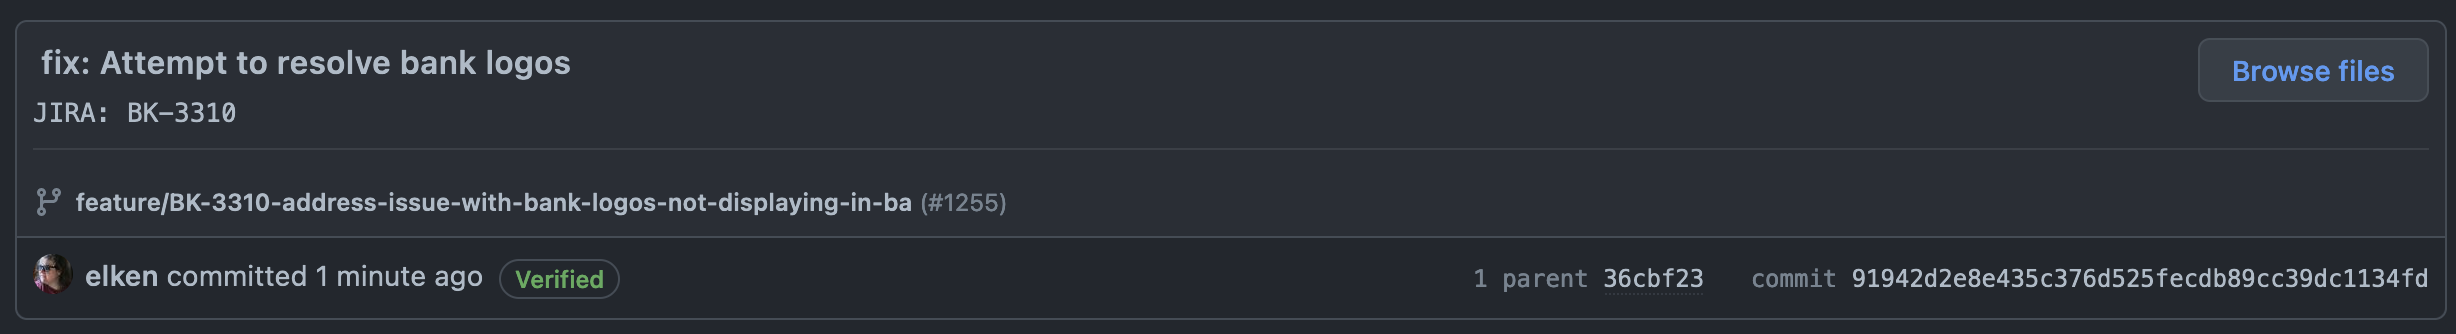
\includegraphics[width=.9\linewidth]{gh_commit.png}
\end{center}
\end{block}

\note{Notes
\tiny

Touched on briefly in the last slide, including the ticket number in the commit message (ideally the footer as not to waste valuable summary space) will link it to the ticket in jira. This also applies to pull requests, and creating a pull request with the ticket ID in square brackets will cause a bot to edit your PR and insert a link to the ticket.
\normalsize}
\end{frame}


\begin{frame}[label={sec:org51e688f}]{When do I commit?}
\begin{itemize}
\item As often as makes sense
\item Avoid massive commits
\item Try and keep a commit for a single feature/bugfix
\end{itemize}

\note{Notes
\tiny

Frequency of commits is another thing to be aware of, committing as often as makes sense will make your life easier so you don't have to undo hundreds of times and will make later reverts much simpler. A good rule of thumb is trying to keep a single logical unit of work to a commit in such a way that if this commit were to be removed, it shouldn't require other commits first.

The \emph{only} exception here is large linting commits, or a gigantic refactor; but in the case of the latter there's probably room to reduce the scope of that ticket.
\normalsize}
\end{frame}

\section{Branches}
\label{sec:org8d34091}
\begin{frame}[label={sec:orgac6fc6c}]{What are they?}
\begin{itemize}
\item A subset of commits
\item A movable pointer
\item \href{https://git-scm.com/book/en/v2/Git-Branching-Branches-in-a-Nutshell}{More info}
\end{itemize}

\note{Notes
\tiny

So we've gone through commits now, the other entity you should be familiar with is branches. Expanding on the previous example, each commit is an object that creates a tree linking it with the previous commit. As you add commits, the pointer for the branch moves forward.

When you make a new branch from a commit or other ref, you create another pointer from which commits can be added to. These branches don't have to be related, and don't even have to contain the same files.

For a deeper dive, see the link on the slide.
\normalsize}
\end{frame}

\section{Conventions}
\label{sec:org7ae5110}
\begin{frame}[label={sec:org9e0f29a},fragile]{Gitflow}
 \begin{itemize}
\item \texttt{<prefix>/<ticket-code>-<trimmed-ticket-desc>}
\begin{itemize}
\item eg \texttt{feature/BK-3310-address-issue-with-...}
\end{itemize}
\item Fixed:
\begin{itemize}
\item \texttt{develop} for the main WIP branch
\item \texttt{staging} for work against a staging server (0 or more per project)
\item \texttt{prod} for live code
\end{itemize}
\item Prefixes:
\begin{itemize}
\item \texttt{feature} for feature development
\begin{itemize}
\item Merge into \texttt{develop}
\end{itemize}
\item \texttt{hotfix} for emergency fixes
\begin{itemize}
\item Merge into \texttt{prod} or \texttt{staging}
\end{itemize}
\item \texttt{release/<semver-num>} for release branches
\end{itemize}
\end{itemize}

\note{Notes
\tiny

Gitflow conventions have already been touched on during the last retro, but just to remind everyone/fill in those who missed it; gitflow is a branch naming model.

In terms of creating branches, there are a number of fixed branches; those being

\begin{itemize}
\item \texttt{develop} for the main WIP branch
\item \texttt{staging} for work against a staging server (of which there could be 0, 1 or many depending on the project)
\item \texttt{prod} for live code (akin to \texttt{master} or \texttt{main} as it is now)
\end{itemize}

In the future, these will ideally be protected in github; meaning the only way to get changes in would be via pull requests (which already require approval from one reviewer).

When dealing with everything else, there is a standard format at the top of the slide (which should be taken care of by the vscode extension that has mentioned before).

\texttt{feature} for branches that revolve around feature work, and \texttt{hotfix} for branches that fix critical issues.
\normalsize}
\end{frame}

\begin{frame}[label={sec:org54ba8ee},fragile]{Forks}
 \begin{itemize}
\item \texttt{origin} for your fork, \texttt{upstream} for the original repo
\begin{itemize}
\item By default pushing goes to your fork
\item Harder to accidentally send commits to the wrong place
\item This is what \texttt{gh} CLI does
\end{itemize}
\item Alternatively \texttt{origin} for the original and \texttt{<gh-username>} for your fork
\begin{itemize}
\item Handles multiple forks
\item Easier to accidentally send commits to the wrong place
\end{itemize}
\end{itemize}

\note{Notes
\tiny

Because of how we primarily use git and github, it's rare we have to handle forks but it's worth covering still.

A fork is simply a copy of a remote repository under a different user. This includes the full history and branches, but doesn't include site-specific things like issues or pull requests.

There are two main ways to handle remote naming with forks, \texttt{origin} for your forked version and \texttt{upstream} for the original version; and \texttt{origin} for the \emph{original} version and the associated github/gitlab/bitbucket owner name (not username because repos can be forked to organisations too).

The first way is the recommended and sensible approach, it's rare you'd be working with multiple forks in the same tree and by default pushes/pulls go to/from your remote repo so there's little chance of pushing changes to the wrong place. This is also how the github CLI tool \texttt{gh} does it, so by using that you're already set.

The other approach is used in a few tools, which typically wrap around git to reduce the chances of pushing to the wrong place; but it could still happen. At the end of the day, neither is strictly better, but I would recommend the first approach.
\normalsize}
\end{frame}

\begin{frame}[label={sec:orgbf9b1fd},fragile]{Upstream}
 \begin{itemize}
\item Provide a MWE (Minimal Working Example)
\item Provide as much info as is pertinent
\item Check for contributor docs
\item Search for issues first to prevent duplication
\end{itemize}

\note{Notes
\tiny

Briefly touched on in the previous slide, there are some things to take into consideration when dealing with upstream.

At the end of the day, a fair percentage of people contributing code are working during their free time so the more you can help them to help you the better.

A good first step is being able to provide a MWE or minimal working example to reproduce the bug. Create a repo if required, but usually just a snippet is enough. Including as much info as you can feeds into this, stack traces, OS name/version, package versions, etc. Whatever is relevant to your issue.

Nowadays if the repo is setup correctly, when making an issue for the first time github will prompt you advising you to read through contributor docs first. This is usually found at the top level but can also exist in a \texttt{docs}  subfolder. This may include code conventions, style guide, how to format commits or PRs, how to reproduce issues, etc.

Lastly, make sure you put at least some effort in trying to find pre-existing issues or related issues. This can save everyone time and creating a new issue when one or even more exist is a good way to get an annoyed response.
\normalsize}
\end{frame}


\section{Usage}
\label{sec:orgf177998}
\begin{frame}[label={sec:org9b04075},fragile]{\texttt{branch}}
 \begin{itemize}
\item \texttt{git checkout -b <name>}
\item \texttt{git checkout <branch>}
\item \texttt{git branch -vv}
\item \texttt{git branch -{}-no-merged} and \texttt{git branch -{}-merged}
\item \texttt{git branch -d <name>}
\end{itemize}

\note{Notes
\tiny

The next few slides will include a couple of relevant commands for the most common operations. First up is branches, and simply we have ``create a branch and set it to be the current branch'', ``checkout another branch'', ``list all branches with more information including which remote branch we're tracking'', ``show me all the branches that have been merged into the default branch'' and vice versa and finally ``delete a branch''.

As with all these slides, you're encouraged to read through the manual pages to see what else is possible.

\normalsize}
\end{frame}

\begin{frame}[label={sec:org558cbf4},fragile]{\texttt{merge}}
 \begin{itemize}
\item \texttt{git checkout branch-to-be-merged-onto \&\& git merge branch-to-merge}
\end{itemize}

\begin{Code}
\begin{Verbatim}
\color{EFD}\textcolor[HTML]{cfd2d6}{here is some content not affected by the conflict}
\colorbox[HTML]{373E4C}{\textcolor[HTML]{aa2222}{<}}\colorbox[HTML]{373E4C}{\textcolor[HTML]{BF616A}{<<<<<< main}}
\textcolor[HTML]{cfd2d6}{this is conflicted text from main}
=======
\textcolor[HTML]{cfd2d6}{this is conflicted text from feature branch}
>>>>>>> feature branch;
\end{Verbatim}
\end{Code}

\note{Notes
\tiny

Next up is merge, and the most common usage. Most git clients have ways to do this easier, along with handling merge conflicts.

A merge conflict is simply just a result of two snapshots affecting the same section and git is unable to decide what should be applied. This is usually a result of not keeping your working branch up-to-date often enough.

Often they have to be resolved manually, but most git clients include some way to resolve these easier.
\normalsize}
\end{frame}


\begin{frame}[label={sec:org8579f93},fragile]{Syncing changes}
 \begin{itemize}
\item \texttt{git fetch}
\item \texttt{git pull}
\item \texttt{git push}
\end{itemize}

\note{Notes
\tiny

Syncing changes mostly revolves around 3 commands; fetch, push and pull.

Fetch will update the current branch (or all refs with \texttt{-{}-all}) by downloading all objects and refs from a remote repo. Note that this won't apply any changes, only the objects.

Related to fetch, we have pull which \emph{will} apply any changes that exist for the currently tracked branch and can also cause merge conflicts.

Last we have push, which will attempt to sync your local changes with changes on a remote repo, if your history is different to what's remote (eg you rebased or you haven't pulled recently) then you'll get an error from the server.
\normalsize}
\end{frame}

\begin{frame}[label={sec:org3b0d4ba},fragile]{\texttt{stash}}
 \begin{itemize}
\item \texttt{git stash}
\item \texttt{git stash pop}
\item \texttt{git stash apply}
\item \texttt{git stash list}
\item \texttt{git stash (pop|apply) <identifier>}
\item \texttt{git stash -p}
\end{itemize}

\note{Notes
\tiny

git stash temporarily shelves (or stashes) changes you've made to your working copy so you can work on something else, and then come back and re-apply them later on. Stashing is handy if you need to quickly switch context and work on something else, but you're mid-way through a code change and aren't quite ready to commit.

So in order we have:

\begin{itemize}
\item ``Stash all changes in my current tree''
\item ``Apply the most recent stash and remove it''
\item ``Apply the most recent stash and \emph{don't} remove it''
\item ``Show me all the stashes in my tree''
\item ``Pop or apply a specific stash based on the identifier (the first column)''
\item ``Interactively decide what to stash''
\end{itemize}

\normalsize}
\end{frame}

\section{Advanced Git}
\label{sec:orgfd73063}
\begin{frame}[label={sec:orgbdd5519}]{Rebase}
\begin{definition}[Rebase]
To reapply a series of changes from a branch to a different base, then reset the head of that branch to the result
\end{definition}

\begin{itemize}
\item Put simply, rewrite history (no DeLoreans here)
\item Can encourage bad habits, especially in a shared environment
\item Destructive action that \emph{\uline{will}} destroy commits
\end{itemize}

\note{Notes
\tiny

OK so we know what commits are now, we know how to write them, what if we make a mistake? I'll just make another commit, right?

Well, as with most guidelines the answer is ``it depends''. If it's just a small thing, you'd probably be better off doing what's called a rebase.

Rebasing is a fancy word with a fancy definition that simply just means writing history. This can be anything from rewording a commit, combining multiple commits together (what's referred to as ``squashing''), adjusting the order of commits and just flat out editing commits.

Using the bare git CLI to rebase can be quite tricky, but tools that wrap around git often include a decent rebase interface. Regardless, the upcoming demo will just use the git CLI.

\normalsize}
\end{frame}


\begin{frame}[label={sec:orgdb0a822},fragile,shrink=40]{Rebase Demo}
 \begin{Code}
\begin{Verbatim}
\color{EFD}\EFt{echo} \EFs{"file"} > file
\EFt{git} add file
\EFt{git} commit -m \EFs{"Added file"}
\end{Verbatim}
\end{Code}

\begin{Code}
\begin{Verbatim}
\color{EFD}\EFrda{[}master 952846e\EFrda{]} Added file
 \EFhn{1} file changed, \EFhn{1} insertion\EFrda{(}+\EFrda{)}
 create mode \EFhn{100644} file
\end{Verbatim}
\end{Code}

\begin{Code}
\begin{Verbatim}
\color{EFD}\EFt{git} log
\end{Verbatim}
\end{Code}

\begin{Code}
\begin{Verbatim}
\color{EFD}commit 952846eda636dc7e6d174fa36b4254aaffdfbb85
Author: Ellis Kenyő <me@elken.dev>
Date:   Wed Nov \EFhn{16} 10:41:15 \EFhn{2022} +0000

    Added file

commit 467b20d4505285307743aa462e213d594851d6c9
Author: Ellis Kenyő <me@elken.dev>
Date:   Wed Nov \EFhn{16} 10:41:15 \EFhn{2022} +0000

    Initial commit
\end{Verbatim}
\end{Code}

\note{Notes
\tiny

The following demo will show how you can use git rebase to reword a commit. The process for more complex interactions like changing commits is quite complex and you're encouraged to either use one of the tools shown later or learn for yourself.

Building on the same repo we made earlier, we only have our initial commit. We can't rebase on more than 1 commit (because there's nothing to rebase \emph{onto}) so we have to just create another commit to let us play with. As before, we're just making a dummy file and committing it.
\normalsize}
\end{frame}


\begin{frame}[label={sec:orgb47ec8b},fragile,shrink=40]{Rebase Demo}
 \begin{columns}
\begin{column}{0.8\columnwidth}
\begin{block}{Pre Rebase}
\begin{Code}
\begin{Verbatim}
\color{EFD}\EFt{git} rebase -i HEAD\char126{}1
\end{Verbatim}
\end{Code}

\begin{center}
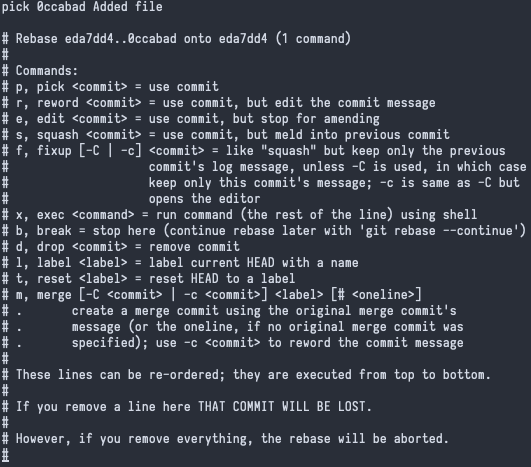
\includegraphics[width=.9\linewidth]{rebase.png}
\end{center}

\begin{center}
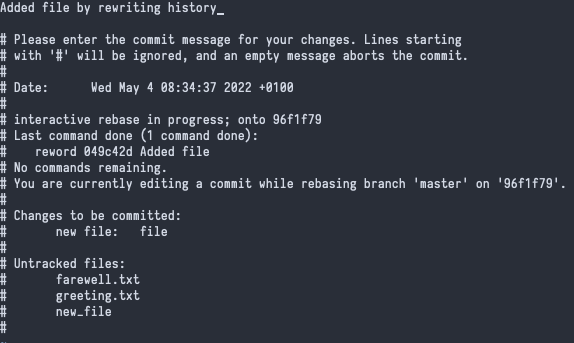
\includegraphics[width=.9\linewidth]{rebase_3.png}
\end{center}
\end{block}
\end{column}

\begin{column}{0.8\columnwidth}
\begin{block}{Post Rebase}
\begin{Code}
\begin{Verbatim}
\color{EFD}\EFt{git} log
\end{Verbatim}
\end{Code}

\begin{Code}
\begin{Verbatim}
\color{EFD}commit 949678607213dea4fefc7bf8632d4a8c648c9293
Author: Ellis Kenyő <me@elken.dev>
Date:   Wed May \EFhn{4} 08:37:53 \EFhn{2022} +0100

    Added file by rewriting history

commit ceab98bd5da79400982df77f6b0120cbacf77fc5
Author: Ellis Kenyő <me@elken.dev>
Date:   Wed May \EFhn{4} 08:37:53 \EFhn{2022} +0100

    Initial commit
\end{Verbatim}
\end{Code}
\end{block}
\end{column}
\end{columns}

\note{Notes
\tiny

Now the process begins, we invoke the command above, which translates to ``\texttt{git rebase} interactively between the most recent commit and the last 1 commit''. In order to perform a rebase, you have to select the range of commits that are to be affected. This can be ``the last 1 commit'' or two specific commit hashes.

In this case though, we're just capturing the last 1 commit.

In the first screenshot, a file has been created and opened in whatever the environment variable \texttt{GIT\_EDITOR} is set to, in this case \texttt{vim}. At the top there is ``pick'' followed by some of the commit hash followed by the message. In the blurb below, all the possible commands are explained.

If we look there, we can see that pick just means ``use this commit'', which means that nothing about it changes and if we were to save this file now, no changes would be made.

As it turns out, we want to change the wording in the commit, so we need to change ``pick'' to ``reword'' and save this file.

After doing that, the bottom screenshot occurs as a new commit message is ready to be written. As you can see in the commented section underneath, this is occurring during an interactive rebase.

After then changing the message and saving this file, the rebase is completed and a fresh \texttt{git log} shows us the new history.
\normalsize}
\end{frame}


\begin{frame}[label={sec:orge68c0e4},fragile]{Rebasing Do's and Don'ts}
 \begin{itemize}
\item \alert{DO} use it sparingly as it's a destructive action
\item \alert{DON'T} use it to amend commits that are far in the past that have been merged
\begin{itemize}
\item In that case, a \texttt{revert} is preferred as it preserves the history while still removing the code
\end{itemize}
\item \alert{DO} be aware that rewriting already pushed commits will require you to force push
\item \uline{\alert{DO} use it sparingly as it's a destructive action}
\end{itemize}

\note{Notes
\tiny

Some guidelines for good rebase usage, do use it sparingly as it's a destructive actions;

\begin{itemize}
\item \alert{DO} use it sparingly as it's a destructive action
\end{itemize}
Reiterating this again because it will wipe your history, and if you haven't synced it remotely it's gone forever.
\begin{itemize}
\item \alert{DON'T} use it to amend commits that are far in the past that have been merged. In that case, a \texttt{revert} is preferred as it preserves the history while still removing the code
\end{itemize}
Self-explanatory, rewriting history is dangerous so using it on anything already pushed is a bad idea. To undo a commit or commits use \texttt{git revert} or whatever your git client of choice has in that area
\begin{itemize}
\item \alert{DO} be aware that rewriting already pushed commits will require you to force push
\end{itemize}
If you are working on a branch that has been synced, and you rebase something, your history and the remote history are now out of sync; so trying to push will result in an error. If this is what you are sure you want to do, the only resolution is to force push which will tell the remote repository you want your changes to take precedence.

This can result in lost work \emph{remotely} and leads on to the last point
\begin{itemize}
\item \uline{\alert{DO} use it sparingly as it's a destructive action}
\end{itemize}
Rebasing and force pushing should only be used for small touch-ups unless you're comfortable with git. If you need to rebase a large PR that has a lot of scattered commits for example, don't be afraid to ask someone senior for help.
\normalsize}
\end{frame}


\section{Closing}
\label{sec:org90f1d4f}
\begin{frame}[label={sec:org8a93bff}]{Clients}
\begin{itemize}
\item \href{https://www.gitkraken.com/}{Gitkraken} (GUI)
\item \href{https://www.sourcetreeapp.com/}{Sourcetree} (GUI)
\item \href{https://desktop.github.com/}{GitHub Desktop} (GUI)
\item \href{https://github.com/jesseduffield/lazygit}{lazygit} (Terminal)
\item \href{https://gitlens.amod.io/}{GitLens} (VSCode)
\end{itemize}

\note{Notes
\tiny

Nearly there now, I've included some recommendations for git clients in no particular order. I've used them all in the past and they're all good, though Gitkraken is what I would consider the most beginner friendly and it also has integrations for jira tickets (GitLens might too and sourcetree ``should'') though it has paid options and I can't comment on how much requires a license now.

Try them all and see what you like more.
\normalsize}
\end{frame}

\begin{frame}[label={sec:org3db9726}]{Thanks for listening!}
\begin{block}{Any questions?}
\end{block}
\end{frame}
\end{document}